\documentclass{article}
\usepackage[utf8]{inputenc}
\usepackage{geometry}
 \geometry{
 a4paper,
 total={170mm,257mm},
 left=20mm,
 top=20mm,
 }
\usepackage{polski}
\usepackage{natbib}
\usepackage[capbesideposition=right]{floatrow}
\usepackage{graphicx}
\usepackage{pbox}
\usepackage{float}
\usepackage[dvipsnames]{xcolor}
\usepackage{caption}
\usepackage{wrapfig}
\usepackage{graphicx}
\usepackage{tikz}
    \usetikzlibrary{
        arrows,
        shadows,
        shapes,
        automata,
        positioning,
        arrows.meta
    }
\usepackage{pgfplots}
\usepackage{tabularx}
\usepackage{booktabs}
\usepackage{amsfonts}
\pgfplotsset{compat=1.17}

\begin{document}
\centering 
\Huge Activity diagram of the simulation 
\vspace{1cm}
\normalsize
    
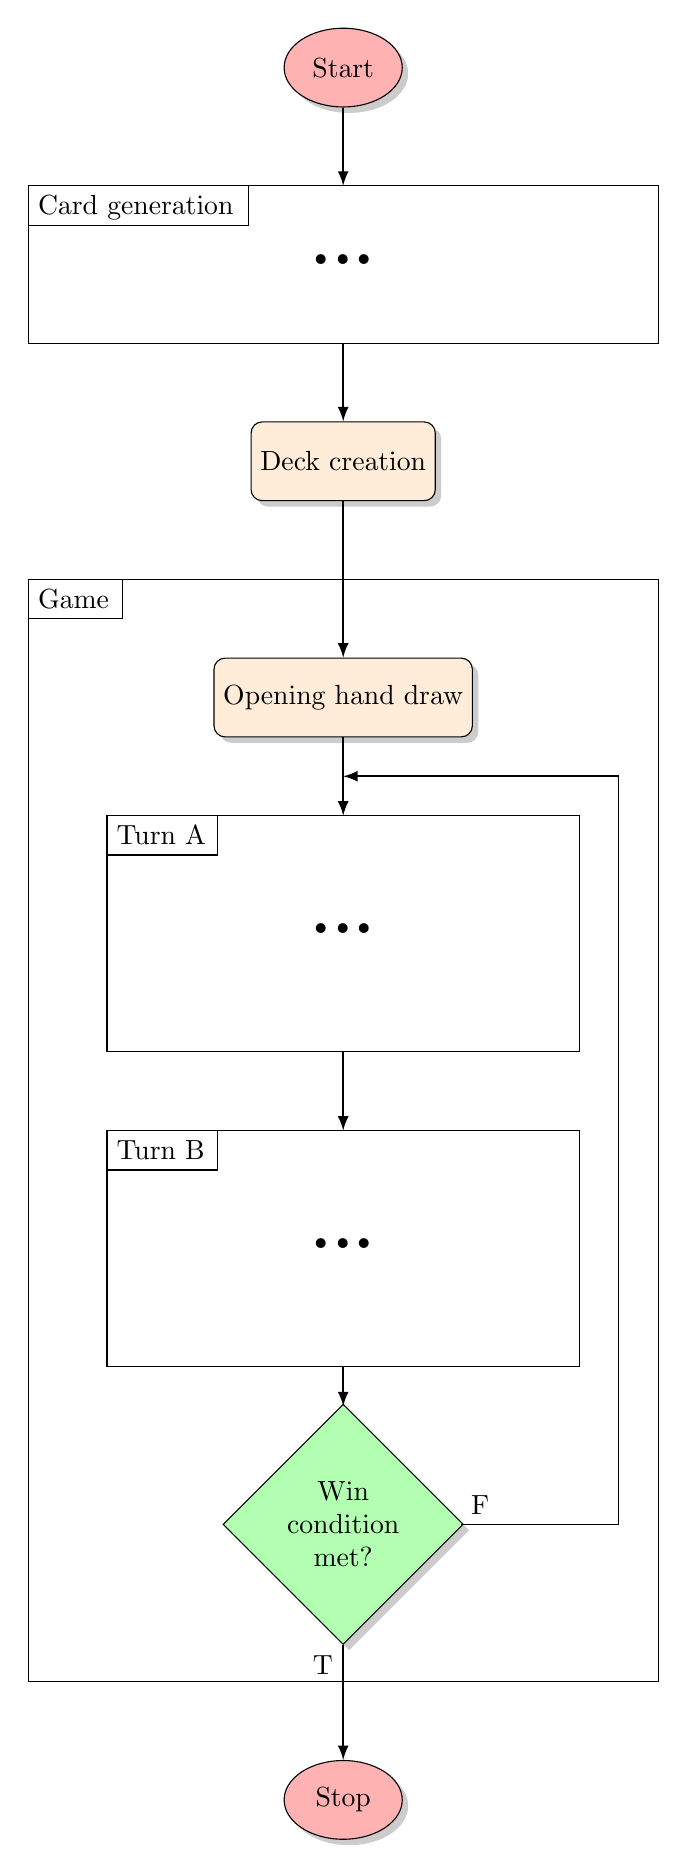
\begin{tikzpicture}
[baseshape/.style={minimum width=1.5cm, minimum height=1cm,text centered, font=\normalsize,draw=black, drop shadow=black!40},
startstop/.style={baseshape, ellipse, fill=red!30},
io/.style={baseshape, trapezium, trapezium stretches=true, 
trapezium left angle=70, trapezium right angle=110, fill=blue!30},
process/.style={baseshape, rectangle, rounded corners, fill=orange!15},
decision/.style={baseshape, diamond, minimum width=1cm, fill=green!30, text width=1.5cm},
block/.style={baseshape, rectangle, minimum width=1cm, fill=white},
arrow/.style={thick, -latex},
node distance=2cm,]

    \node (step0) [startstop, yshift= 0.5cm ] {Start}; 
    \node (step1) [process, below of= step0, yshift = -3cm] {Deck creation};
    \node (step2) [process, below of= step1, yshift = -1cm] {Opening hand draw};
    \node (step4) [decision, below of = step1, yshift = -11.5cm] {Win \\ condition \\ met?};
    \node (step5) [startstop, below of = step4, yshift = -1.5cm] {Stop};
    
    \draw[arrow] (step0) -- (0, -1);
    \draw[arrow] (0, -3) -- (step1);
    \draw[arrow] (step1) -- (step2);
    \draw[arrow] (step2) -- (0, -9);
    \draw (1.5, -18) -- node[at start, anchor=south west]{F}(3.5, -18) -- (3.5, -8.5);
    \draw[arrow] (3.5, -8.5) -- (0, -8.5);
    \draw[arrow] (0, -12) -- (0, -13);
    \draw[arrow] (0, -16) -- (0, -16.5);
    \draw[arrow] (step4) -- node[at start, anchor=north east]{T}(step5);
    
    \draw (-4,-1) -- node[at start, anchor=north west]{Card generation}(-1.2,-1) -- (-1.2, -1.5) -- (-4, -1.5) -- node[at start, anchor=north, yshift = -0.25cm, xshift = 4cm]{\Huge{\textbf{...}}}(-4, -1) -- (4, -1) -- (4, -3) -- (-4,-3) -- (-4, -1);
    \draw (-4,-6) -- node[at start, anchor=north west]{Game}(-2.8,-6) -- (-2.8, -6.5) -- (-4, -6.5) -- (-4, -6) -- (4, -6) -- (4, -20) -- (-4,-20) -- (-4, -6);
    \draw (-3,-9) -- node[at start, anchor=north west]{Turn A}(-1.6,-9) -- (-1.6, -9.5) -- (-3, -9.5) -- node[at start, anchor=north, yshift = -0.75cm, xshift = 3cm]{\Huge{\textbf{...}}}(-3, -9) -- (3, -9) -- (3, -12) -- (-3,-12) -- (-3, -9);
    \draw (-3,-13) -- node[at start, anchor=north west]{Turn B}(-1.6,-13) -- (-1.6, -13.5) -- (-3, -13.5) -- node[at start, anchor=north, yshift = -0.75cm, xshift = 3cm]{\Huge{\textbf{...}}}(-3, -13) -- (3, -13) -- (3, -16) -- (-3,-16) -- (-3, -13);
\end{tikzpicture}
\end{document}